\section{Optimierung der Parameter der Likelihood-Methode}
Um den AMS-Wert zu erhöhen, wurden drei der Parameter der Likelihood-Methode innerhalb folgender Grenzen variiert:

\begin{equation}
\begin{split}
\mbox{\textit{PDFInterpol}} &\in \{ \mbox{ Spline0,  Spline1, \ldots, Spline5}  \}  \\
 \mbox{\textit{NSmooth}} &\in \{ \mbox{0, 1, \ldots, 12} \} \\
  \mbox{\textit{NAvEvtPerBin}} &\in \{ \mbox{38, 39, \ldots, 52} \} \\
\end{split}
\end{equation}

Die Verteilung der erzielten AMS-Werte ist  Abbildung \ref{fig:likelihood_hist} zu entnehmen.
Da auch bei diesem Verfahren die erzielten AMS-Werte deutlich unter $0,5$ blieben, entschieden wir uns dafür, auch diesen Algorithmus in der weiteren Analyse nicht weiter zu verwenden.


\begin{figure}[htp]
\begin{center}
  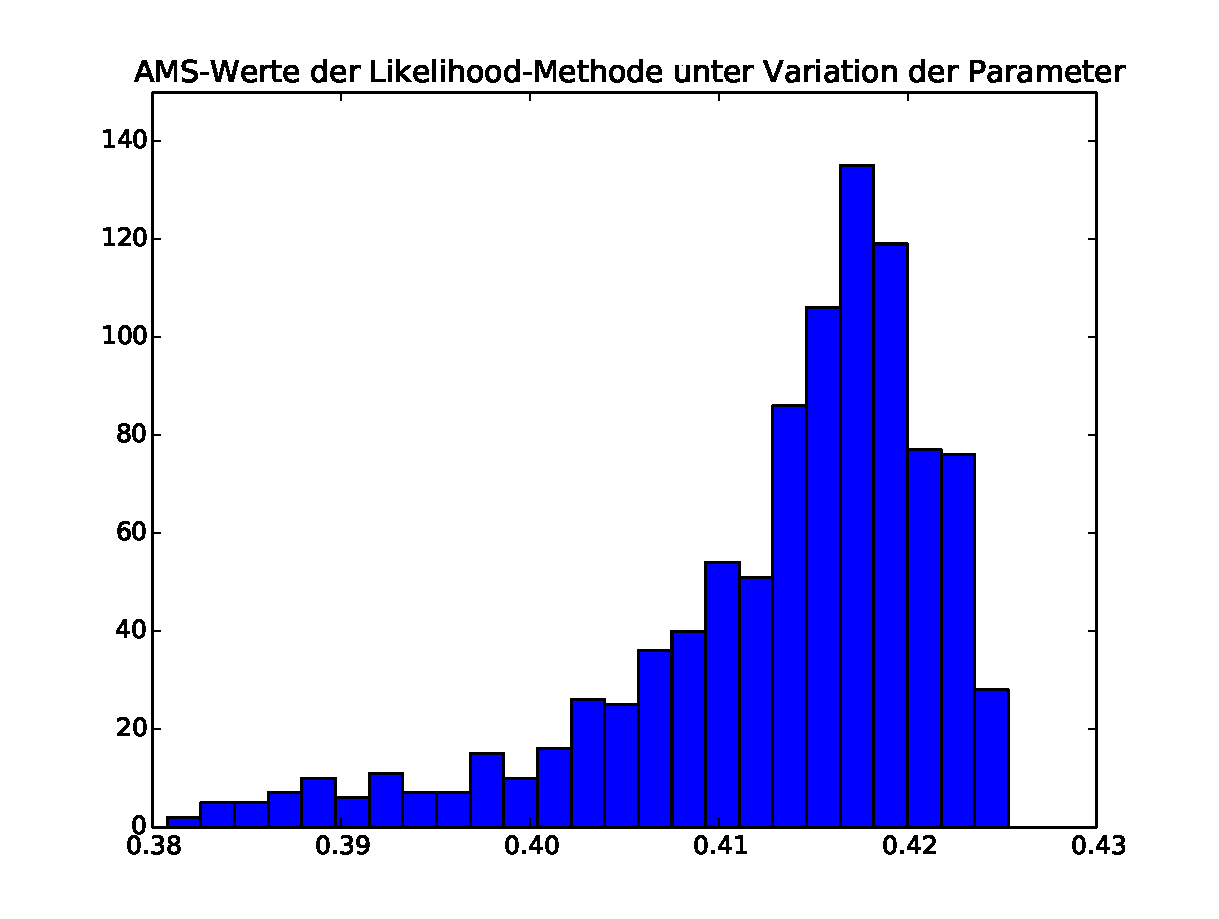
\includegraphics[width=0.7\linewidth]{sections/parameter_optimization_likelihood/likelihood_AMS_hist.pdf}
 \caption[Histogramm der erzielten AMS-Werte]{Histogramm der erzielten AMS-Werte.}
\label{fig:likelihood_hist}
\end{center}
\end{figure}